\documentclass[aspectratio=169, 10pt]{beamer}

\usepackage{bm} % bold math
\usepackage{fontspec}
\usepackage{minted}
\usepackage{pgf-pie}
\usepackage{tikz}
\usepackage{graphicx}
\newcommand\sbullet[1][.5]{\mathbin{\vcenter{\hbox{\scalebox{#1}{$\bullet$}}}}}

% Custom commands and environments
\makeatletter
\newcommand\version[1]{\renewcommand\@version{#1}}
\newcommand\@version{}
\def\insertversion{\@version}

\newcommand\course[1]{\renewcommand\@course{#1}}
\newcommand\@course{}
\def\insertcourse{\@course}

\newcommand\coursetitle[1]{\renewcommand\@coursetitle{#1}}
\newcommand\@coursetitle{}
\def\insertcoursetitle{\@coursetitle}

\newcommand\lecturenumber[1]{\renewcommand\@lecturenumber{#1}}
\newcommand\@lecturenumber{}
\def\insertlecturenumber{\@lecturenumber}
\makeatother

\newcommand{\slidetitle}[1]{{\xbseries \large \structure{#1}} \bigskip}
\newcommand{\term}[1]{{\color{blue} #1}}
\newcommand{\leftspace}{\hspace{1em}}
\newcommand{\inlinearrow}{
  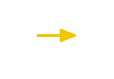
\begin{tikzpicture}[baseline]
    \node [anchor=base] (x) {};
    \draw [rawarrow] (x.mid west) -- ($(x.mid west) + (2em,0)$);
  \end{tikzpicture}
}

\newenvironment{slide}
{\begin{frame}[fragile,environment=slide]\vskip0pt plus 1filll}
{\vskip0pt plus 1filll\end{frame}}

% LaTeX

\setlength{\leftmargini}{1em}

% Common Information

\author{Talia Xu}
\course{COMPSCI 340}
\coursetitle{Operating Systems}
\date{2024 Semester 2}

% fontspec

\defaultfontfeatures{Ligatures=TeX}
% \setmainfont{Domine}
\setsansfont{Inter}[
  FontFace={ul}{n}{Font=*-Thin},
  FontFace={el}{n}{Font=*-ExtraLight},
  FontFace={l}{n}{Font=*-Light},
  FontFace={sb}{n}{Font=*-SemiBold},
  FontFace={eb}{n}{Font=*-ExtraBold},
  FontFace={xb}{n}{Font=*-Black},
]
\setmonofont[Contextuals=AlternateOff, Ligatures=TeXOff]{Iosevka}[
  FontFace={xb}{n}{Font=*-Heavy},
]

%% Font Weights

\DeclareRobustCommand{\ulseries}{\fontseries{ul}\selectfont}
\DeclareTextFontCommand{\textul}{\ulseries}
\DeclareRobustCommand{\elseries}{\fontseries{el}\selectfont}
\DeclareTextFontCommand{\textel}{\elseries}
\DeclareRobustCommand{\lseries}{\fontseries{l}\selectfont}
\DeclareTextFontCommand{\textl}{\lseries}
\DeclareRobustCommand{\sbseries}{\fontseries{sb}\selectfont}
\DeclareTextFontCommand{\textsb}{\sbseries}
\DeclareRobustCommand{\ebseries}{\fontseries{eb}\selectfont}
\DeclareTextFontCommand{\texteb}{\ebseries}
\DeclareRobustCommand{\xbseries}{\fontseries{xb}\selectfont}
\DeclareTextFontCommand{\textxb}{\xbseries}

% tikz

\usetikzlibrary{
  arrows,
  arrows.meta,
  automata,
  backgrounds,
  calc,
  decorations.pathreplacing,
  matrix,
  positioning,
  overlay-beamer-styles,
  shapes,
  shapes.multipart,
  tikzmark,
}

\tikzstyle{rawarrow} = [
  -{Latex[round]},
  line width=1pt,
  yellow,
  shorten >=3pt,
  shorten <=3pt,
  font=\small,
  text=black,
]

\tikzstyle{arrow} = [
  -{Latex[round]},
  line width=1pt,
  yellow,
  shorten >=3pt,
  shorten <=3pt,
  transform canvas={yshift=3pt},
  font=\small,
  text=black,
]

\newcommand{\tikzmarkcoord}[1]{([yshift=3pt]pic cs:#1)}

% minted

\setminted{style=eyolfson, fontsize=\small, escapeinside=||}
\setmintedinline{fontsize=\normalsize}

% hyperref

\hypersetup{colorlinks, urlcolor=blue}

% beamer
\setbeamersize{text margin left=16mm, text margin right=16mm}
\setbeamertemplate{itemize items}[circle]
\setbeamercolor{item}{fg=black}
\setbeamercolor{structure}{fg=darkblue}
\setbeamerfont{frametitle}{series=\bfseries, parent=structure}
\setbeamertemplate{navigation symbols}{}
\setbeamertemplate{headline}{}
\setbeamertemplate{footline}{
  \begin{tikzpicture}[
    remember picture,
    overlay,
    shift={(current page.south west)},
  ]
    \path [fill=gray] (144mm, 0) -- (160mm, 16mm) -- (160mm, 0);
    \node [inner sep=3.5mm, outer sep=0, text=black, anchor=base east,
           align=right, yshift=3.5mm]
          at (current page.south east) {\ttfamily \small \insertframenumber{}};
  \end{tikzpicture}
}
\setbeamertemplate{title page}{
  \begin{tikzpicture}[
    remember picture,
    overlay,
    shift={(current page.south west)},
    background rectangle/.style={fill=darkblue},
    show background rectangle,
  ]
    \node [anchor=center, align=center, text=white, text width=40mm, scale=3.2]
          at (\paperwidth / 2, \paperheight * 2 / 3)
          {\xbseries \inserttitle{}};
    \node [anchor=base west, align=left, inner sep=0, text=white, yshift=2.5mm]
          at (16mm, \paperheight / 3)
          {\insertdate{} \insertcourse{}: \insertcoursetitle{}};
    \node [anchor=base west, align=left, inner sep=0, text=white, yshift=-2.5mm]
          at (16mm, \paperheight / 3)
          {\insertauthor};
    \node [anchor=base east, align=right, inner sep=0, text=white, yshift=2.5mm]
          at (144mm, \paperheight / 3)
          {Lecture \insertlecturenumber{}};
    \node [anchor=base east, align=right, inner sep=0, text=white,
           yshift=-2.5mm]
          at (144mm, \paperheight / 3)
          {\ttfamily \insertversion{}};
    \node [align=center, anchor=south, inner sep=0, text=white, yshift=3.5mm]
          (license) at (\paperwidth / 2, 0)
          {\fontsize{7pt}{7pt}\selectfont This  work is licensed under a
           \href{http://creativecommons.org/licenses/by-sa/4.0/}
                {\color{lightblue} Creative Commons Attribution-ShareAlike 4.0
                 International License}};
  \end{tikzpicture}
}

% xcolor

%% Primary Colour

\definecolor{pantone655}{RGB}{0, 42, 92} % #002a5c
\colorlet{darkblue}{pantone655}

%% Secondary Colours

\definecolor{pantone633}{RGB}{0, 139, 176} % #008bb0
\colorlet{blue}{pantone633}

\definecolor{pantonewarmred}{RGB}{220, 70, 51} % #dc4633
\colorlet{red}{pantonewarmred}

\definecolor{pantone3285}{RGB}{0, 161, 137} % #00a189
\colorlet{cyan}{pantone3285}

\definecolor{pantone7722}{RGB}{13, 83, 77} % #0d534d
\colorlet{darkcyan}{pantone7722}

\definecolor{pantone376}{RGB}{141, 191, 46} % #8dbf2e
\colorlet{green}{pantone376}

\definecolor{pantone2613}{RGB}{109, 36, 122} % #6d247a
\colorlet{violet}{pantone2613}

\definecolor{pantone2985}{RGB}{111, 199, 234} % #6fc7ea
\colorlet{lightblue}{pantone2985}

\definecolor{pantone227}{RGB}{171, 19, 104} % #ab1368
\colorlet{magenta}{pantone227}

\definecolor{pantone7406}{RGB}{241, 197, 0} % #f1c500
\colorlet{yellow}{pantone7406}

%% Neutrals

\definecolor{pantonecoolgray2}{RGB}{208, 209, 201} % #d0d1c9
\colorlet{gray}{pantonecoolgray2}


\lecturenumber{1}
\title{File\\Systems}
\version{1.0.0}

\begin{document}

\begin{frame}[plain, noframenumbering]
    \titlepage
\end{frame}

\begin{slide}

    \slidetitle{What can happen on a crash?}

    Assume we are creating and writing to a new file /foo/bar

    Write in general (not just the first write)
    \medskip

    \includegraphics[width=130mm]{system-crash-1.png}

\end{slide}

\begin{slide}

    \slidetitle{What can happen on a crash?}
    
    Assume we are creating and writing to a new file /foo/bar
    \bigskip

    A crash after the completion of:
    \begin{itemize}
        \item Step   1-5: No corruption.
        \item Step     6: i-node bitmap points to garbage data.
        \item Step   7-9: Inconsistent metadata.
        \item Step 10-12: No corruption.  
        \item Step    13: data bitmap points to garbage data.
        \item Step    14: Corrupted data.
        \item Step    15: The new data cannot be found. 
    \end{itemize}

\end{slide}


\begin{slide}
    
    \slidetitle{What can happen on a crash?}

    \textbf{Lost Files:} New files being created might not be fully registered in the directory structure, leading to them being "lost" even if their data exists on disk.
    \bigskip

    \textbf{Inaccessible Files:} Existing files might become inaccessible due to corrupted metadata or lost pointers to their data blocks.
    \bigskip
    
    \textbf{Incorrect File Sizes:} The file system might report incorrect file sizes due to incomplete writes or metadata updates.
    \bigskip

    \textbf{Inconsistent Metadata:} Applications trying to access affected files might crash, freeze, or produce errors due to the inconsistencies.

\end{slide}

\begin{slide}

    \slidetitle{Recovery from failure}

    \textbf{Consistency checking} compares data in directory structure with data blocks on disk, and tries to fix inconsistencies.
    \begin{itemize}
        \item Tools: fsck for Unix systems, chkdsk for Windows.
        \item Scanning the entire disk, slow, very slow ...
    \end{itemize}
    \bigskip

    \textbf{Journaling:} A system that keeps track of changes that will be made in the file system to ensure data integrity.
    \bigskip

    \textbf{Versioning and Snapshots:} Maintain historical versions or states of files and systems to roll back when needed.
    \bigskip

    \textbf{Backup and Restore:} Periodic backups to external devices or cloud storage, ensuring data can be restored from a known good state.

\end{slide}

\begin{slide}

    \slidetitle{Journaling (a.k.a Write-Ahead Logging)} 

    Used by many modern file systems: 
    \begin{itemize}
        \item Linux (ext3, ext4), Windows (NTFS), IBM (JFS)
    \end{itemize}
    \bigskip

    First write down what you are going to do, and then carry out the action
    \bigskip

    \includegraphics[width=80mm]{journaling-1.png}
    \medskip

    \includegraphics[width=80mm]{journaling-2.png}

\end{slide}

\begin{slide}

    \slidetitle{Journaling (a.k.a Write-Ahead Logging)} 

    Physical journal
    \begin{itemize}
        \item all changed data is recorded in the journal first
    \end{itemize}
    \bigskip

    Logical journal
    \begin{itemize}
        \item only changed metadata (like inode tables, directory structures) is recorded
    \end{itemize}

\end{slide}

\begin{slide}

    \slidetitle{Journaling (a.k.a Write-Ahead Logging)} 

    What if absolute data integrity is crucial?
    \begin{itemize}
        \item for example, in banking, aviation systems, stock exchange?
    \end{itemize}
    \bigskip
    
    How do we ensure that data integrity is always maintained?

\end{slide}

\begin{slide}

    \slidetitle{ZFS}
    
    What happens if system crashes before each step can be completed?
    \bigskip

    \includegraphics[width=65mm]{zfs.jpg}

\end{slide}

\begin{slide}

    \slidetitle{Why distributed system? An example}

    2004: Facebook started on a single server
    \begin{itemize}
        \item Web server front end to assemble each user’s page. 
        \item Database to store posts, friend lists, etc.
    \end{itemize}
    \medskip

    2008: 100M users
    \medskip

    2010: 500M users
    \medskip

    2012: 1B users
    \medskip

    2019: 2.5B users
    \medskip

\end{slide}

\begin{slide}

    \slidetitle{Why distributed system?}

    Nature of the application
    \begin{itemize}
        \item Multiplayer games
        \item Collaborative Projects \& Cloud App
    \end{itemize}
    \bigskip

    Availability despite unreliable components 
    \begin{itemize}
        \item A service shouldn’t fail when one computer does. • 
    \end{itemize}
    \bigskip

    Conquer geographic separation 
    \begin{itemize}
        \item A web request in NZ is faster served by a server in NZ than by a server in US.
    \end{itemize}
    \bigskip

    Scale up capacity 
    \begin{itemize}
        \item More CPU cycles, more memory, more storage
    \end{itemize}

\end{slide}

\begin{slide}

    \slidetitle{What is a distributed system?}

    \begin{exampleblock}{}
          {\large ``A collection of loosely coupled nodes interconnected by a communication network.''}
            \vskip5mm
              \hspace*\fill{\small--- textbook}
    \end{exampleblock}

\end{slide}

\begin{slide}

    \slidetitle{What is a distributed system?}

    \includegraphics[width=65mm]{dfs-definition-1.png}
    \bigskip

    \textbf{Independent components or elements}
    \begin{itemize}
        \item software processes or hardware used to run a process, store data, etc.
    \end{itemize}

\end{slide}

\begin{slide}

    \slidetitle{What is a distributed system?}

    \includegraphics[width=65mm]{dfs-definition-2.png}
    \bigskip

    \textbf{Independent components or elements} that are \textbf{connected by a network.}

\end{slide}

\begin{slide}

    \slidetitle{What is a distributed system?}

    \includegraphics[width=80mm]{dfs-definition-4.png}
    \bigskip

    \textbf{Independent components or elements} that are \textbf{connected by a network} and \textbf{communicate by passing messages} to achieve a common goal, appearing as \textbf{a single coherent system}.
    \bigskip

    When one (or more) component fails, the system does not fail.

\end{slide}

\begin{slide}

    \slidetitle{The client-server model}

    \includegraphics[width=80mm]{client-server-model.png}
    \bigskip

    Unstructured communication 
    \begin{itemize}
        \item Use shared memory or shared data structures
    \end{itemize}

    Structured communication 
    \begin{itemize}
        \item Message-oriented model
    \end{itemize}

\end{slide}

\end{document}
